\documentclass[12pt]{article}
\usepackage{graphicx}
\usepackage{wrapfig}
\usepackage{subfigure}
\usepackage{multirow}
\usepackage{hyperref}
\usepackage{amsmath}
\usepackage{amssymb}
%\usepackage{ngerman}
\usepackage[ansinew]{inputenc}
\usepackage[left=2cm,top=1cm]{geometry}

% vector graphics test
\usepackage{color}
\usepackage{transparent}
\graphicspath{{graphs/}}

\setlength{\parindent}{0pt}

%\usepackage[outdir=./]{epstopdf}
%\epstopdfsetup{outdir=./}


\begin{document}
	\pagestyle{empty}
	

\begin{titlepage}
	\centering
	\bigskip
	\huge{Astronomisches Praktikum: Altersbestimmung offener Sternhaufen}\\
	\bigskip
	\large{Versuch 4}\\
	\bigskip
	\large{Jan R\"{o}der \& Julia Lienert}
	\bigskip
	\tableofcontents
\end{titlepage}

\pagebreak


\section{Einleitung}

Entstehen viele Sterne am selben Ort zur (fast) gleichen Zeit, resultiert das in der Entstehung eines offenen Sternhaufens. Typische Massen betragen ca. 1000\,M$_\odot$; besteht er aus Riesensternen, kann ein offener Haufen mit einigen Millionen Jahren kurzlebig sein, aber auch sehr langlebig, wenn er z. B. aus M-Sternen besteht.\\
Tr\"{a}gt man die Sterne eines Sternhaufens in ein Hertzsprung-Russell-Diagramm ein, stellt man fest, dass es eine Art ``Abknickpunkt'', oder ``Turnover'' gibt. Anhand dieses Punktes kann man das Alter des Haufens bestimmen, denn der Sternhaufen ist umso j\"{u}nger, desto h\"{o}her dieser Punkt im Diagramm liegt. Man kann ausserdem die Temperatur und Masse von Sternen im Haufen berechnen, wenn man den ``Turnover'' kennt. \\
In diesem Versuch sind scheinbare Helligkeiten und Farbindizes von Sternen eines unbekannten Haufens gegeben, aus denen obengenannte Gr\"{o}ssen bestimmt werden sollen, um herauszufinden, um welchen Haufen es sich handelt.


\section{Analyse eines unbekannten Sternhaufens}

\subsection{Aufgabe 1}
\begin{figure} [h]
	\centering
	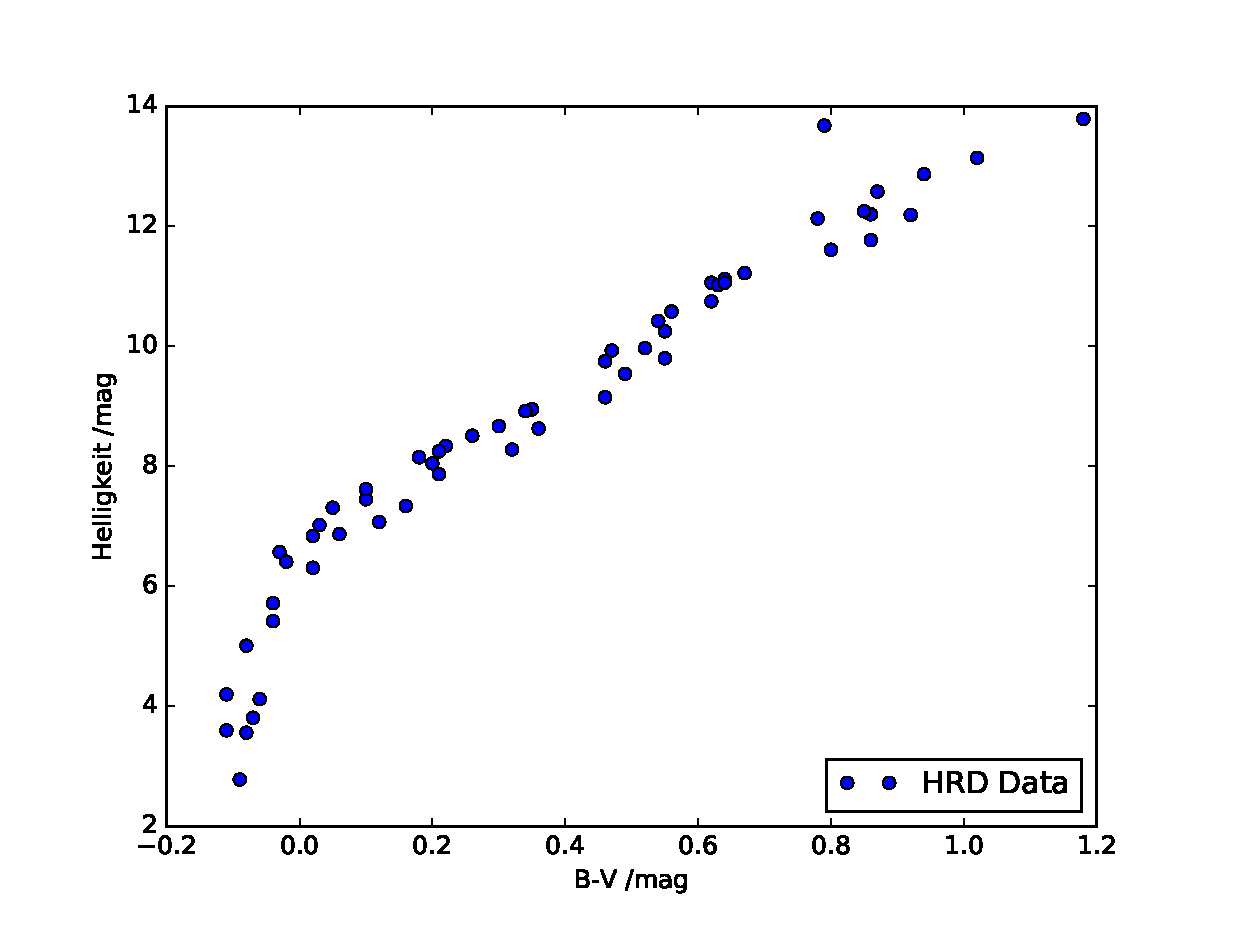
\includegraphics[width=1\textwidth]{hrd_notitle.eps}
	\caption{Scheinbare Helligkeit und Farbindex gegeneinander aufgetragen. Der rote Punkt w\"{a}re die Sonne, w\"{a}re sie Teil des Haufens.}
	\label{fig:hrd_unknown}
\end{figure}

Im Diagramm sind die Werte aus Tabelle 4.1 der Anleitung aufgetragen. Die Hauptreihe knickt bei ca. $m=6$\,mag und $B-V=-0.01$\,mag ab.

\subsection{Aufgabe 2}

Abbildung 4.2 der Anleitung zeigt die abolute Helligkeit aufgetragen gegen den Farbindex, f\"{u}r einige bekannte Sternhaufen. Hier kann man anhand des Farbindexes das ALter des unbekannten Sternhaufens ablesen. Alternativ kann der Farbindex in die effektive Temperatur umgerechnet werden, um Abbildung 4.3 b) verwenden zu k\"{o}nnen. Ohne Information \"{u}ber die Entfernung des Haufens k\"{o}nnen die y-Achsen der Graphen, die jeweils die abolute Helligkeit darstellen, nicht verwendet werden. \\
Die hellsten Sterne sind oft blaue Riesensterne, die eine Farbe zwischen weisslichem Blau und Blau haben. Das entspricht einem Farbindex von etwa $-0.2$.

\subsection{Aufgabe 3}

Der Abknickpunkt f\"{u}r $B-V\simeq -0.01$\,mag steht hier f\'{u}r ein Alter von etwa $10^8$ Jahren (Plejaden in Abb. 4.2). 

\subsection{Aufgabe 4} \label{dist}

Liest man in Abb. 4.2 die zum bestimmten Farbindex geh�rende abolute Helligkeit ab, kann man sie zusammen mit der scheinbare Helligkeit des Abknickpunkts in das Entfernungsmodul einsetzen. Man erh�lt aus der Abbildung $M\simeq 0.5$\,mag.
\begin{align*}
	r &= 10\text{\,pc} \cdot 10^{\frac{m-M}{5}} = 10\text{\,pc} \cdot 10^{\frac{5.5}{5}} \\
	r &\simeq 125.89\text{\,pc} 
\end{align*}

\subsection{Aufgabe 5}

Das Alter von $10^8$ Jahren ergibt $\log t = 8$, mithilfe von Abbildung 4.3 b) erh�lt man dann $\log \,T_{eff}=4.05$ (der x-Wert zu dem Abknickunkt der Kurve, die zu $\log t = 8$ geh�rt, von der ZAMS.) Damit ist $T_{eff} \simeq 11\,221$\,K. Dies wiederum liefert den x-Wert zu der Kurve zum gesuchten $\log M/M_\odot$ in Abbildung 4.3 a). Man kann $\log M/M_\odot = 0.4$ ablesen, bzw. $M\simeq 2.51$\,M$_\odot$. Der abzulesende Wert ist hier wieder der Abknickpunkt der Kurve vom \"{A}quivalent der ZAMS-Kurve im $\log L/L_\odot$-$\log T_{eff}$-Diagramm.

\subsection{Aufgabe 6}

Der Entfernung nach zu Urteilen handelt es sich vermutlich um die Plejaden bei $r \simeq 136$\,pc. Unser Wert ist $10$\,pc zu niedrig, gleicht jedoch den vom Hipparcos-Satelliten bestimmten $125$\,pc im Jahr 1999. \\
Das Alter der Plejaden mit rund $100$\,Mio. Jahren stimmt gut mit der Literatur \"{u}berein.




\section{Hertzsprung-Russell-Diagramme}

\subsection{Aufgabe 1}

Die Sonne wird insgesamt etwa $11$\,Mrd. Jahre ein Hauptreihenstern sein. Ihr momentanes Alter betr\"{a}gt rund $4.57$\,Mrd. Jahre. \\
Die Lebensdauer eines Sterns h\"{a}ngt im Wesentlichen von der Masse und dem Energieertrag ab. Letzterer ist die Bilanz aus der gesamten im Sterninneren produzierten Energie und der Strahlungsenergie, die abgestrahlt wird. Der Energieertrag ist somit eine erste, grobe Absch\"{a}tzung f\"{u}r die Lebensdauer. \\
Die absolute Helligkeit der Sonne betr\"{a}gt $M=4.83$\,mag; der hellste Stern im Datensatz hat $M=-2.72$\,mag. Er ist damit wesentlich leuchtkr\"{a}ftiger als die Sonne. Ausserdem ist er weiss-bl\"{a}ulich, w\"{a}hrend die Sonne ein gelblicher Stern ist. Der hellste Stern des Datensatzes wird deutlich weniger Zeit auf der Hauptreihe verbringen. \\
Mit den Gleichungen 
\begin{align}
	\frac{L}{L_\odot} &= 10^{-0.4\,(M-M_\odot)} \label{eq:LL10MM} \\
	L &\sim M^{7/2} \label{eq:prop}\\
	\tau_{HR} &\sim 10^{10}\text{\,yr} \cdot \left(\frac{M}{M_\odot}\right)\left(\frac{L_\odot}{L}\right) = 10^{10}\text{\,yr} \cdot \left(\frac{L_\odot}{L}\right)^{7/2} \label{eq:time}
\end{align}
kann man absch\"{a}tzen, dass der hellste Stern des Datensatzes nur knapp $70$\,Mio. Jahre lang ein Hauptreihenstern ist. Bei Gleichungen \ref{eq:prop} und \ref{eq:time} ist hier zu beachten dass $M$ Massen bezeichnen. In Gleichung \ref{eq:LL10MM} ist $M$ die absolute Helligkeit. Formel \ref{eq:prop} bezeichnet man auch als Masse-Leuchtkraft-Beziehung; Formel \ref{eq:time} ermittelt eine Absch\'{a}tzung f\"{u}r die Hauptreihen-Lebensdauer basierend auf dem Wert f\"{u}r die Sonne.


\subsection{Aufgabe 2}

In Abbildung \ref{fig:hrd_unknown} ist die Sonne als roter Punkt basierend auf dem in \ref{dist} ermittelten Abstand eingetragen. Ihre scheinbare Helligkeit w\"{u}rde etwa $m_\odot\simeq 10$\,mag betragen; mit dem blossen Auge sind Sterne aber nur bis $m=6$\,mag sichtbar. Man k\"{o}nnte die Sonne also nicht mit dem Auge sehen, st\"{u}nde sie in dem unbekannten Sternhaufen.

\subsection{Aufgabe 3} 
\begin{figure}[h]
	\centering
	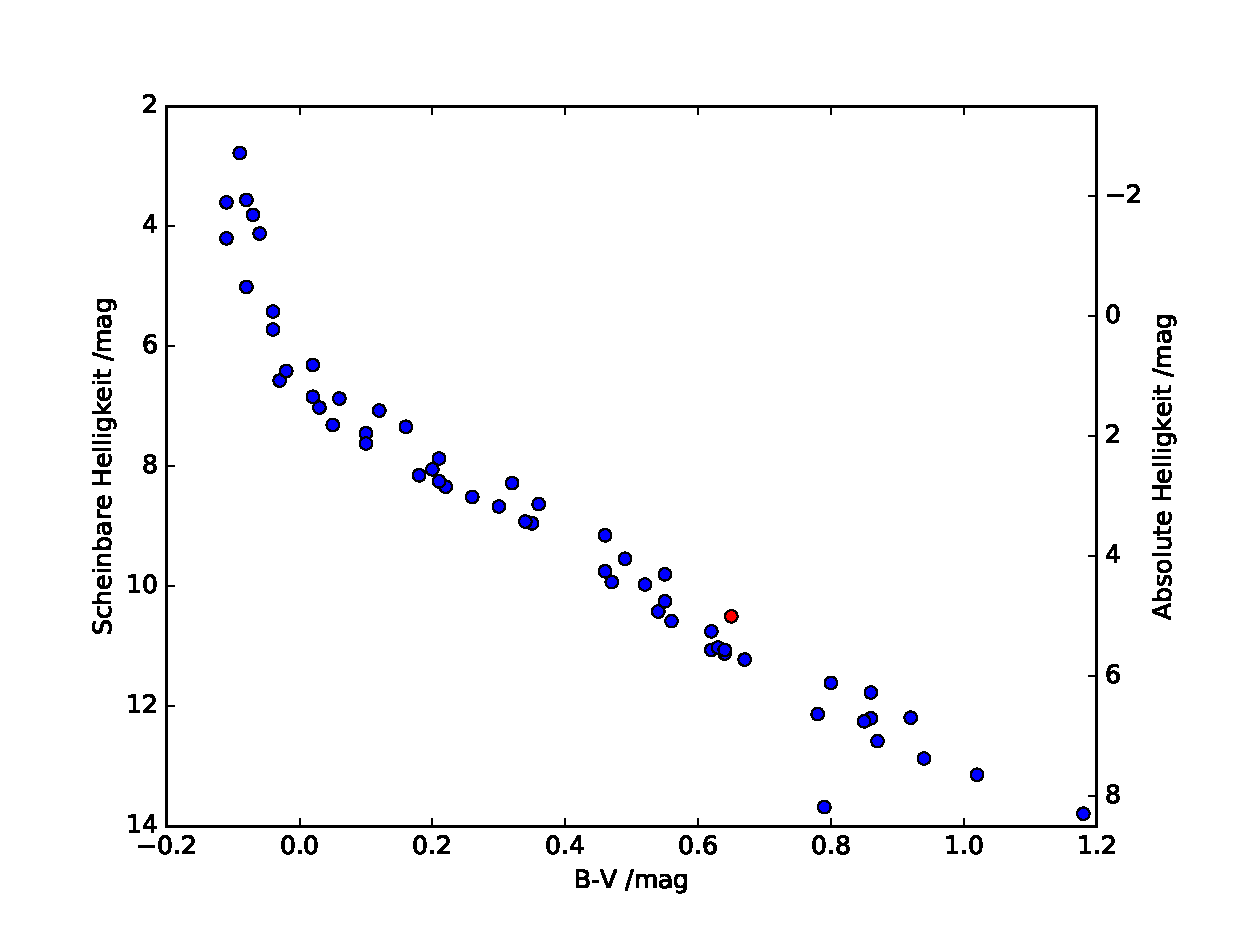
\includegraphics[width=1\textwidth]{hrd_twoy.eps}
	\caption{Scheinbare und absolute Helligkeit gegen Farbindex aufgetragen}
	\label{fig:hrd_twoy}
\end{figure}

Da alle Sterne im Haufen in etwa den gleichen Abstand zu uns haben, kann man mit dem Entfernungsmodul $m-M=const.$ annehmen und somit die rechte y-Achse generieren, indem man die linke Achse um diesen konstanten Wert (hier ca. $5.5$) nach unten verschiebt. 
\begin{equation*}
	m-M\simeq 5\text{\,mag} \cdot \log\left(\frac{126\text{\,pc}}{10\text{\,pc}}\right)\simeq 5.5\text{\,mag}
\end{equation*}
Damit ergibt sich Abbildung \ref{fig:hrd_twoy}.

\subsection{Aufgabe 4}

W\"{a}hlt man am Himmel per Zufall Sterne aus und tr\"{a}gt sie in ein $T$-$m$-Diagramm ein, so l\"{a}sst man ausser Acht, wie weit sie entfernt sind. Dieses Diagramm hat somit keine charakteristische Struktur. Erst wenn man $m$ in $M$ umrechnet und ein $T$-$M$-Diagramm erstellt, sieht es aus wie ein HRD, da nun alle Helligkeiten normiert wurden. Alternativ kann man auch, wie in diesem Versuch, nur Sterne aus einem Abstand in ein $T$-$m$-Diagramm eintragen, dass dann direkt die gewohnte Struktur aufweist.

\pagebreak

\section{Diskussion}

Wenn die Werte auch signifikante Ungenauigkeiten aufweisen, so war es doch m\"{o}glich, den unbekannten Sternhauen als die Plejaden zu identifizieren. Unser Ergebnis f\"{u}r den Abstand wich 10\,pc ab, lag jedoch \"{u}berraschend nah an dem des Hipparcos-Satteliten. Mithilfe der gegebenen Diagramme war es gut m\"{o}glich, die effektive Temperatur und die Masse der Sterne am Abknickpunkt zu bestimmen.\\
Im zweiten Versuchsteil wurden dann noch die Lebensdauer von Sternen auf der Hauptreihe sowie die Eigenschaften verschiedener HRD-Varianten untersucht und das im ersten Teil gezeichnete Diagramm um eine weitere y-Achse f\"{u}r die absolute Helligkeit erweitert. Hier wurde ausgenutzt, dass alle Sterne in einem Sternhaufen n\"{a}herungsweise denselben Abstand zu uns haben.


















\end{document}